\documentclass[10pt,a4paper]{article}
\usepackage[margin=20mm,top=18mm,bottom=19mm]{geometry}
\usepackage[T1]{fontenc}
\usepackage{lmodern,microtype}
\usepackage{amsmath,amssymb,booktabs,tabularx,array,multirow}
\usepackage{graphicx,xcolor,tikz}
\usetikzlibrary{arrows.meta,positioning}
\usepackage[font=small,labelfont=bf]{caption}
\usepackage[numbers,sort&compress]{natbib}
\usepackage{enumitem,fancyhdr}
\usepackage[hidelinks,breaklinks]{hyperref}
\usepackage{xurl}
\definecolor{navy}{RGB}{28,56,85}
\hypersetup{pdftitle={Reproducing ACE and Evaluating Diagnostic-Free Offline Training on Formula},pdfauthor={WANG Haowei}}
\newcommand{\reportauthor}{WANG Haowei}
\newcommand{\studentid}{1155244499}

\setlength{\parindent}{0pt}
\setlength{\parskip}{4pt}
\setlength{\emergencystretch}{2em}
\setlength{\tabcolsep}{5pt}
\renewcommand{\arraystretch}{1.15}
\newcolumntype{Y}{>{\raggedright\arraybackslash}X}
\newcolumntype{P}[1]{>{\raggedright\arraybackslash}p{#1}}
\newcommand{\art}[1]{\texttt{\small\detokenize{#1}}}
\newcommand{\pp}{\,\mathrm{pp}}
\newcommand{\smalltable}{\small\setlength{\tabcolsep}{4pt}}
\setlist[itemize]{leftmargin=*,nosep,topsep=3pt}
\pagestyle{fancy}\fancyhf{}
\fancyhead[L]{\small FTEC5660 Reproducibility Work}
\fancyhead[R]{\small ACE on Formula}
\fancyfoot[C]{\thepage}
\setlength{\headheight}{14pt}
\title{\vspace{-13mm}\LARGE\bfseries Reproducing ACE and Evaluating\\Diagnostic-Free Offline Training on Formula}
\author{\reportauthor\quad (\studentid)\\\small Agentic AI for Business and FinTech (FTEC5660)}
\date{10 November 2026}
\begin{document}
\maketitle\thispagestyle{fancy}
\vspace{-5mm}
\begin{abstract}
\noindent This study evaluates Agentic Context Engineering (ACE) on financial numerical reasoning using the authors' implementation and a resource-constrained DeepSeek Flash configuration. On 100 official test questions evaluated under three training-order seeds, ACE attains 84.00\% accuracy versus 69.33\% for an empty-playbook Generator, a difference of 14.67 percentage points. A subsequent execution optimization removes a training-time answer used exclusively for diagnostic measurement. Fixed-response replay preserves all 180 learning states, six validation checkpoints and three selected playbooks. Three fresh paired training runs reduce learning calls by 23.51\% and cache-aware learning-cost estimates by 17.87\%. On a separate 160-question project holdout, both conditions obtain 86.46\% accuracy, but the question-clustered 95\% difference interval, $[-2.08,+2.08]$ percentage points, does not meet the predefined lower-bound criterion. The evidence supports behavioral reproduction and observed efficiency benefits, while remaining insufficient to establish accuracy preservation. Auxiliary experiments and implementation deviations are reported rather than omitted.
\end{abstract}
\section{Introduction and Reproduction Target}
Financial question answering requires both appropriate formulas and reliable numerical execution. This project asks whether accumulated textual experience improves performance, and whether training overhead can be reduced without deleting learning opportunities. It reproduces one offline Formula task using the public ACE implementation, rather than attempting every benchmark or updating model weights.

\begin{table}[h!]
\centering\smalltable
\begin{tabularx}{\linewidth}{P{10mm}YY}
\toprule
 & Research question & Evaluation \\
\midrule
RQ1 & Does learned context improve accuracy? & ACE vs. empty playbook \\
RQ2 & Can diagnostic calls be removed? & Replay and fresh training \\
RQ3 & Is accuracy preserved? & Prespecified holdout audit \\
\bottomrule
\end{tabularx}
\caption{Three questions separating behavior, efficiency and accuracy.}
\end{table}
The principal modification is diagnostic-free \emph{offline execution}, not a new learning algorithm. Earlier selective-reflection, retrieval and output-policy studies remain part of the record. The report's focus evolved after those studies; it is not presented as the project's sole original hypothesis. Code, protocols, selected playbooks and public measured outputs accompany the report~\cite{thisrepo}.

\clearpage
\section{System, Reference Result, and Experimental Setup}
\subsection{Reproduced system and comparison boundary}
ACE uses a Generator, Reflector and Curator to maintain an evolving textual playbook. Learning changes context rather than model weights~\cite{zhang2026ace}. The official implementation is retained at upstream revision \art{82709de050e1db6e6ef2f07bcb0393560b94992a}~\cite{acerepo}; the added experimental harness resides in \art{repro/}. Formula data, preprocessing, prompts used by the original condition, and numeric scoring are preserved.

\begin{table}[h!]
\centering\smalltable
\begin{tabularx}{\linewidth}{Y Y rr}
\toprule
Source & Model & Baseline (\%) & ACE with labels (\%) \\
\midrule
Paper, Table 2~\cite{zhang2026ace} & DeepSeek-V3.1 & 67.5 & 85.5 \\
This study, test A & DeepSeek Flash & 69.33 & 84.00 \\
\bottomrule
\end{tabularx}
\caption{Reference results and local reproduction. Cross-study differences are not controlled.}
\label{tab:reference}
\end{table}
Our baseline uses the upstream ACE Generator with an empty playbook; the paper's Base LLM uses dataset-default prompts. Differences in backbone, scale and baseline prompts preclude strict numerical replication of the paper's 85.5\% result. The defensible target is the \emph{behavior} that learned context improves performance under the local setup. A difference between the paper's number and ours cannot be attributed to any single cause.

\subsection{Execution configuration}
\begin{table}[h!]
\centering\smalltable
\begin{tabularx}{\linewidth}{P{37mm}Y}
\toprule
Component & Setting \\
\midrule
Runtime & macOS; Python 3.12.13; upstream \art{uv.lock} \\
Model & DeepSeek; \art{deepseek-flash} \\
Endpoint & \url{https://api.deepseek.com} \\
Decoding & Temperature 0; thinking off; 4,096-token cap \\
Output settings & JSON mode off; provider-default \art{top_p} \\
Training & 60 questions; one epoch; up to three reflection rounds \\
Curation & Every training sample \\
Validation & 30 questions; checkpoints at steps 30 and 60 \\
Order seeds & 42, 43, 44 \\
Book selection & Best validation checkpoint \\
Integrity & Frozen hashes; released labels \\
\bottomrule
\end{tabularx}
\caption{Shared configuration. Exact parameters and hashes are in the study manifests.}
\end{table}
Inference is hosted; the local machine performs orchestration without GPU training. The requested and returned model alias is \art{deepseek-flash}; \art{top_p} is not explicitly set. Order seeds control sample order, not server-side randomness. Keys remain in an ignored local \art{.env}; public usage excludes keys and request headers, and raw archives remain local. Dataset, source, template and playbook hashes are frozen before each evaluation.

The original release contains 500/300/200 train/validation/test questions. A separate 10-train/10-validation pilot checked execution and budgeting; both pilot conditions scored 6/10. The formal 60/30/100 scale was selected from cost projections before test scoring, not from accuracy.

\clearpage
\section{Evaluation Design and Accounting}
\subsection{Cohorts and prospective controls}
\begin{table}[h!]
\centering\smalltable
\begin{tabularx}{\linewidth}{P{20mm}Y Y P{34mm}}
\toprule
Study & Questions & Workload & Purpose \\
\midrule
Initial & Official test A: 100 & Five conditions; 1,500 outputs & Behavior and ablations \\
V2 & Validation: 20 + 40; test B: 100 & 600 test outputs & Brief-output selection and test \\
V3 & Development: 40; train/validation: 60/30 & 240 dev outputs; six training runs & Routing; fresh training \\
V4 & Validation-derived holdout: 160 & Six fixed books; 960 outputs & Accuracy audit \\
\bottomrule
\end{tabularx}
\caption{Distinct cohorts and workloads. Accuracy comparisons remain within each study.}
\end{table}
The prespecified initial modification contrast was combined minus ACE. V2 screened candidates on 20 validation questions, confirmed one on 40, and locked it before the disjoint test B. The six V3 training runs separately reused the original 60/30 training/validation split.

V3 reserved 160 validation-pool questions after allocating 40 to routing development. The routing candidate failed its gate and was never evaluated on that holdout. V4 later used the 160 questions for a separately frozen comparison of the six V3-selected training artifacts. All six prediction files were completed and hash-locked before unified scoring. A prior bulk-parsing deviation is disclosed in Section~\ref{sec:limits}.

\subsection{Accuracy and uncertainty}
Let $a_{is}^{(m)}$ be the correctness indicator for question $i$, order seed/playbook $s$, and condition $m$. We report mean accuracy and paired difference as
\[
\widehat A_m=\frac{1}{3N}\sum_{i=1}^{N}\sum_{s=1}^{3}a_{is}^{(m)},\qquad
\widehat\Delta=\frac{1}{N}\sum_{i=1}^{N}\frac{1}{3}\sum_{s=1}^{3}\big(a_{is}^{(\mathrm{modified})}-a_{is}^{(\mathrm{original})}\big).
\]
The unchanged scorer removes commas and compares parsed floats exactly, with string equality as fallback; no tolerance or percentage normalization is added. Missing or unparseable answers remain in the denominator. Nonempty truncated responses follow the upstream parser and are flagged.

Confidence intervals use 10,000 paired question-cluster bootstrap resamples with RNG seed 2026. Each sampled question retains its three paired book outputs. Thus, V4 has 160 independent question units, not 480 independent questions per condition. Intervals condition on the selected books; they do not capture all variability from arbitrary future retraining. Reported SD is sample SD across the three order-seed/book accuracies.

\subsection{Cost and latency definitions}
For completed requests with recorded usage, uncached input $U$, cached input $H$ and output tokens $O$ give the frozen estimate
\[
C_{\mathrm{CNY}}=\frac{8}{10^6}\left(0.30U+0.006H+1.20O\right).
\]
Rates are peak USD prices per million tokens~\cite{deepseekpricing}; factor 8 is a conservative accounting coefficient, not an observed exchange rate. Standardized cost prices all input as uncached. Actual cache reuse can differ across conditions~\cite{deepseekcache}. Unknown-billing reserves are added separately where applicable. Estimates are not reconciled provider bills. Training, selection validation and inference are separated. API time and end-to-end wall time are observational, not service-independent benchmarks.

\clearpage
\section{Modification: Diagnostic-Free Offline Execution}
\subsection{Isolation and preserved learning behavior}
Source inspection of \art{ACE._train_single_sample} identified an extra Generator answer after reflection and curation. This \art{_post_curate} answer measures post-update training accuracy; it does not modify the playbook, global entry IDs or the next sample's learning input. Checkpoint selection uses separate validation.

\begin{figure}[h!]
\centering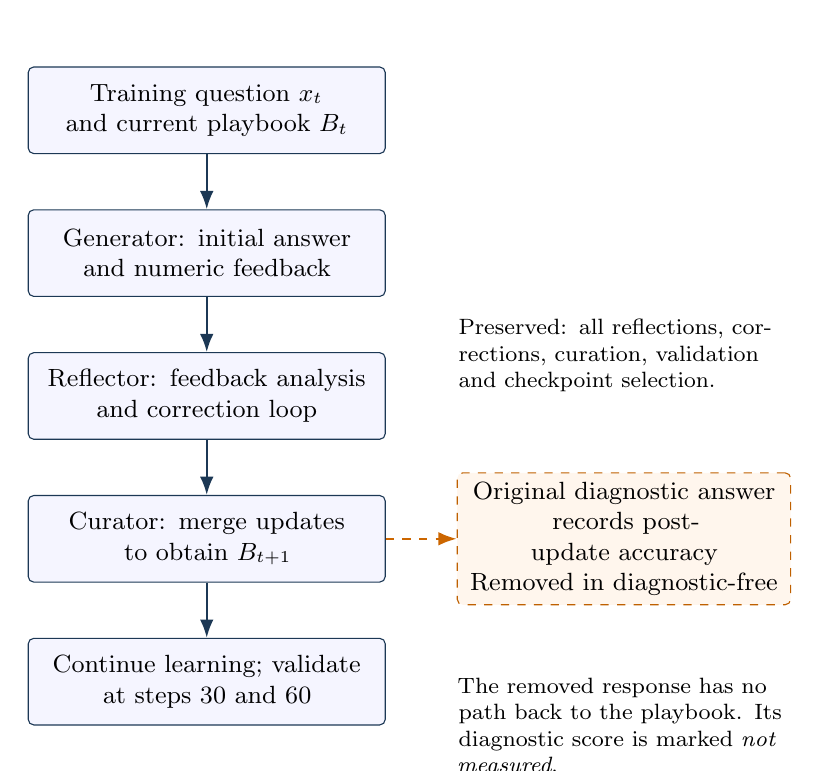
\begin{tikzpicture}[>=Latex, node distance=7mm and 9mm,
 stagebox/.style={draw=navy, rounded corners=2pt, fill=blue!4, align=center, font=\small, text width=43mm, minimum height=11mm},
 note/.style={draw=orange!75!black, dashed, rounded corners=2pt, fill=orange!7, align=center, font=\small, text width=40mm, minimum height=13mm},
 arr/.style={->, thick, draw=navy}]
\node[stagebox] (input) {Training question $x_t$\\and current playbook $B_t$};
\node[stagebox, below=of input] (gen) {Generator: initial answer\\and numeric feedback};
\node[stagebox, below=of gen] (reflect) {Reflector: feedback analysis\\and correction loop};
\node[stagebox, below=of reflect] (curate) {Curator: merge updates\\to obtain $B_{t+1}$};
\node[stagebox, below=of curate] (next) {Continue learning; validate\\at steps 30 and 60};
\node[note, right=of curate] (diag) {Original diagnostic answer\\records post-update accuracy\\Removed in diagnostic-free};
\draw[arr] (input)--(gen); \draw[arr] (gen)--(reflect); \draw[arr] (reflect)--(curate); \draw[arr] (curate)--(next);
\draw[->, dashed, thick, orange!80!black] (curate)--(diag);
\node[align=left, font=\footnotesize, text width=42mm, above=9mm of diag] {Preserved: all reflections, corrections, curation, validation and checkpoint selection.};
\node[align=left, font=\footnotesize, text width=42mm, below=8mm of diag] {The removed response has no path back to the playbook. Its diagnostic score is marked \emph{not measured}.};
\end{tikzpicture}

\caption{The isolated change removes the dashed diagnostic branch. Solid arrows retain the learning and selection path. The diagram describes this project's offline driver, not an arbitrary online ACE deployment.}
\label{fig:flow}
\end{figure}
The diagnostic-free driver skips only that branch. It retains reflection on correct examples, corrections on incorrect examples, all Curator updates and checkpoint validation. A skipped score is \emph{null/not measured}, rather than zero or a copy of the initial score. Consequently, the custom driver also handles missing diagnostic statistics; inserting null into the unchanged upstream accuracy aggregation would be invalid. This intervention is distinct from selective reflection, which removes learning opportunities. It is not applicable where the post-update answer is itself the required online task output.

\subsection{Fixed-response replay evidence}
\begin{table}[h!]
\centering\smalltable
\begin{tabularx}{\linewidth}{Y P{55mm}}
\toprule
Replay check & Result \\
\midrule
Learning states & 180/180 identical \\
Entry IDs and initial answers & Match at every step \\
Validation checkpoints & 6/6 identical \\
Selected playbooks & 3/3 hashes identical \\
New API calls & 0 \\
\bottomrule
\end{tabularx}
\caption{State equivalence under fixed retained responses.}
\end{table}
Each retained request is checked against the archived model, prompt, role, ID and parameter fingerprints. Public findings are in \art{diagnostic_free_replay.json}; full replay requires excluded local archives.

This establishes equivalence \emph{conditional on identical retained responses}. It does not establish byte-identical fresh hosted-model runs, unchanged cache behavior, or universal accuracy preservation. Those questions require separate measurements.

\clearpage
\section{Results I: ACE Behavior Reproduction}
\begin{table}[h!]
\centering\smalltable
\begin{tabularx}{\linewidth}{Yrrr}
\toprule
Condition & Seed accuracy (\%) & Mean $\pm$ SD (\%) & Correct / total \\
\midrule
Empty playbook & 68 / 71 / 69 & $69.33\pm1.53$ & 208/300 \\
Original ACE & 81 / 85 / 86 & $84.00\pm2.65$ & 252/300 \\
Selective reflection & 78 / 81 / 80 & $79.67\pm1.53$ & 239/300 \\
ACE + TF-IDF retrieval & 84 / 80 / 80 & $81.33\pm2.31$ & 244/300 \\
Selective + retrieval & 84 / 83 / 80 & $82.33\pm2.08$ & 247/300 \\
\bottomrule
\end{tabularx}
\caption{Test A: 100 questions per seed, ordered 42/43/44.}
\label{tab:reproduction}
\end{table}
All conditions use the same 100 questions and three order seeds. Retrieval uses the original learned books; the combined condition uses selectively learned books.

ACE improves over the empty-playbook Generator by $14.67\pp$, with a question-clustered 95\% interval of $[8.33,21.67]\pp$. This supports the targeted behavior under the changed backbone and reduced scale. It does not establish that the paper's full experimental result has been reproduced numerically.

\begin{table}[h!]
\centering\smalltable
\begin{tabularx}{\linewidth}{Yrr}
\toprule
Contrast & Difference (pp) & 95\% CI (pp) \\
\midrule
ACE minus empty playbook & +14.67 & [8.33, 21.67] \\
Selective minus ACE & -4.33 & [-7.33, -1.67] \\
Retrieval minus ACE & -2.67 & [-5.67, -0.33] \\
Combined minus ACE (primary) & -1.67 & [-3.67, +0.33] \\
\bottomrule
\end{tabularx}
\caption{Paired differences on test A.}
\end{table}
The primary combined-minus-ACE contrast is negative in point estimate. Other ablation contrasts are exploratory, without multiplicity adjustment.

Selective reflection preserves the original loop for incorrect initial answers but retains reflection/curation for only every fifth correct example. TF-IDF retrieval selects at most 12 entries under a 1,500-token budget for inference. These interventions reduce learning or context volume, but none outperforms original ACE on this cohort.

\subsection{Why token reduction is not sufficient}
\begin{table}[h!]
\centering\smalltable
\begin{tabularx}{\linewidth}{Yrr}
\toprule
Metric & Original ACE & Combined \\
\midrule
Cache-aware inference cost (CNY) & 0.530 & 0.597 \\
Standardized inference cost (CNY) & 1.889 & 0.631 \\
Input cache hit (\%) & 94.7 & 22.0 \\
Cache-aware learning + inference (CNY) & 2.606 & 1.657 \\
\bottomrule
\end{tabularx}
\caption{Estimated costs per book plus 100 answers. Learning excludes validation.}
\end{table}
The combined method reduces standardized learning and inference costs, yet its cache-aware inference cost is higher. Variable retrieved prefixes and lower observed cache reuse are consistent with this discrepancy, but caching and interruptions were not independently controlled. Thus, the full cost difference is not causally attributable to retrieval alone. These results motivated an alternative that preserves learning opportunities and complete inference context.

\clearpage
\section{Results II: Fresh Training Efficiency}
Six fresh jobs compare original and diagnostic-free training using the same original 60/30 adaptation split and paired order seeds. A first seed-42 pair and budget check precede seeds 43 and 44. Condition order alternates across seeds. The original historical books remain unchanged; these jobs produce six new selected books.

\begin{table}[h!]
\centering\smalltable
\begin{tabularx}{\linewidth}{Yrrr}
\toprule
Metric & Original & Diagnostic-free & Change \\
\midrule
Learning calls & 787 & 602 & $-23.51\%$ \\
Diagnostic calls & 180 & 0 & $-100\%$ \\
Retained calls & 607 & 602 & $-0.82\%$ \\
Cache-aware learning cost (CNY) & 5.9796 & 4.9114 & $-17.87\%$ \\
Standardized learning cost (CNY) & 8.4772 & 5.9641 & $-29.64\%$ \\
Workflow cost (CNY) & 6.5203 & 5.5716 & $-14.55\%$ \\
Learning cache hit & 43.5\% & 27.3\% & $-16.2\pp$ \\
Median workflow time (s) & 788.6 & 646.2 & $-18.06\%$ \\
\bottomrule
\end{tabularx}
\caption{Fresh training: three runs pooled; workflow time is the median. Workflow includes validation.}
\label{tab:fresh}
\end{table}
\begin{table}[h!]
\centering\smalltable
\begin{tabularx}{\linewidth}{Yrrrr}
\toprule
Seed & \multicolumn{2}{c}{Learning cost (CNY)} & \multicolumn{2}{c}{Workflow time (s)}\\
\cmidrule(lr){2-3}\cmidrule(lr){4-5}
 & Original & Diagnostic-free & Original & Diagnostic-free \\
\midrule
42 & 1.5885 & 1.6084 & 656.9 & 646.2 \\
43 & 2.1009 & 1.8678 & 788.6 & 685.8 \\
44 & 2.2902 & 1.4352 & 851.0 & 602.2 \\
\bottomrule
\end{tabularx}
\caption{Per-seed cache-aware cost and workflow time.}
\end{table}
The seed-42 diagnostic-free learning-cost estimate is slightly higher than the original estimate. All costs in this section are usage-based estimates rather than reconciled bills; learning excludes selection-validation calls.

Removing 180 measurement-only calls is structurally interpretable. The net difference of 185 learning calls also includes five fewer retained calls in fresh trajectories. Hosted responses and correction loops may differ even at temperature zero, and cache hits fall from 43.5\% to 27.3\%. Therefore, the entire observed cost reduction is not a controlled estimate of the diagnostic branch's isolated causal cost. Three pairs support a local efficiency observation, not a universal savings guarantee.

Validation scores selected the books and are not independent evidence of accuracy. The replay result establishes a fixed-response invariant; Table~\ref{tab:fresh} measures fresh execution. Neither replaces a held-out quality comparison.

\subsection{Combined training and inference accounting}
Adding V3 training plus validation to V4 inference gives CNY 8.2839 for original training versus CNY 7.2661 for diagnostic-free training, a 12.29\% reduction. This is an assembled cross-stage estimate for three trained books and 160 answers per book, not a single uninterrupted deployment bill. Training and inference percentage savings must not be added. The quality qualification in the following section applies to this comparison.

\clearpage
\section{Results III: Fixed-Book Holdout Accuracy Audit}
V4 compares the six books selected in V3 without retraining or replacing them. Each condition answers the same 160 validation-derived holdout questions with the original Generator prompt and full book. No routing, brief-output policy or fallback is used. Seeds 42 and 44 run the original condition first; seed 43 reverses the order. Each job is serial, with three job queues in parallel. Labels enter scoring only after all prediction artifacts are locked.

\begin{table}[h!]
\centering\smalltable
\begin{tabularx}{\linewidth}{Yrr}
\toprule
Metric & Original & Diagnostic-free \\
\midrule
Correct / total & 415/480 & 415/480 \\
Accuracy $\pm$ SD (\%) & $86.46\pm1.30$ & $86.46\pm2.53$ \\
Seed accuracy (\%) & 86.88 / 85.00 / 87.50 & 83.75 / 88.75 / 86.88 \\
Inference cost / 100 answers (CNY) & 0.3674 & 0.3530 \\
Output tokens & 130,977 & 123,150 \\
Finite numeric output (\%) & 98.5 & 98.8 \\
Truncated responses & 8 & 6 \\
API median / P95 (s) & 1.456 / 4.316 & 1.432 / 3.862 \\
\bottomrule
\end{tabularx}
\caption{V4: 480 outputs per condition; seed order 42/43/44. Costs are cache-aware estimates.}
\end{table}
\begin{table}[h!]
\centering\smalltable
\begin{tabularx}{\linewidth}{Y r r P{23mm}}
\toprule
Criterion & Minimum (pp) & Observed (pp) & Decision \\
\midrule
Point difference & $-1$ & $0.00$ & Pass \\
95\% CI lower bound & $-2$ & $-2.0833$ & Fail \\
Overall & \multicolumn{2}{c}{Both criteria required} & Not met \\
\bottomrule
\end{tabularx}
\caption{Prespecified operational accuracy checks.}
\end{table}
\begin{figure}[h!]
\centering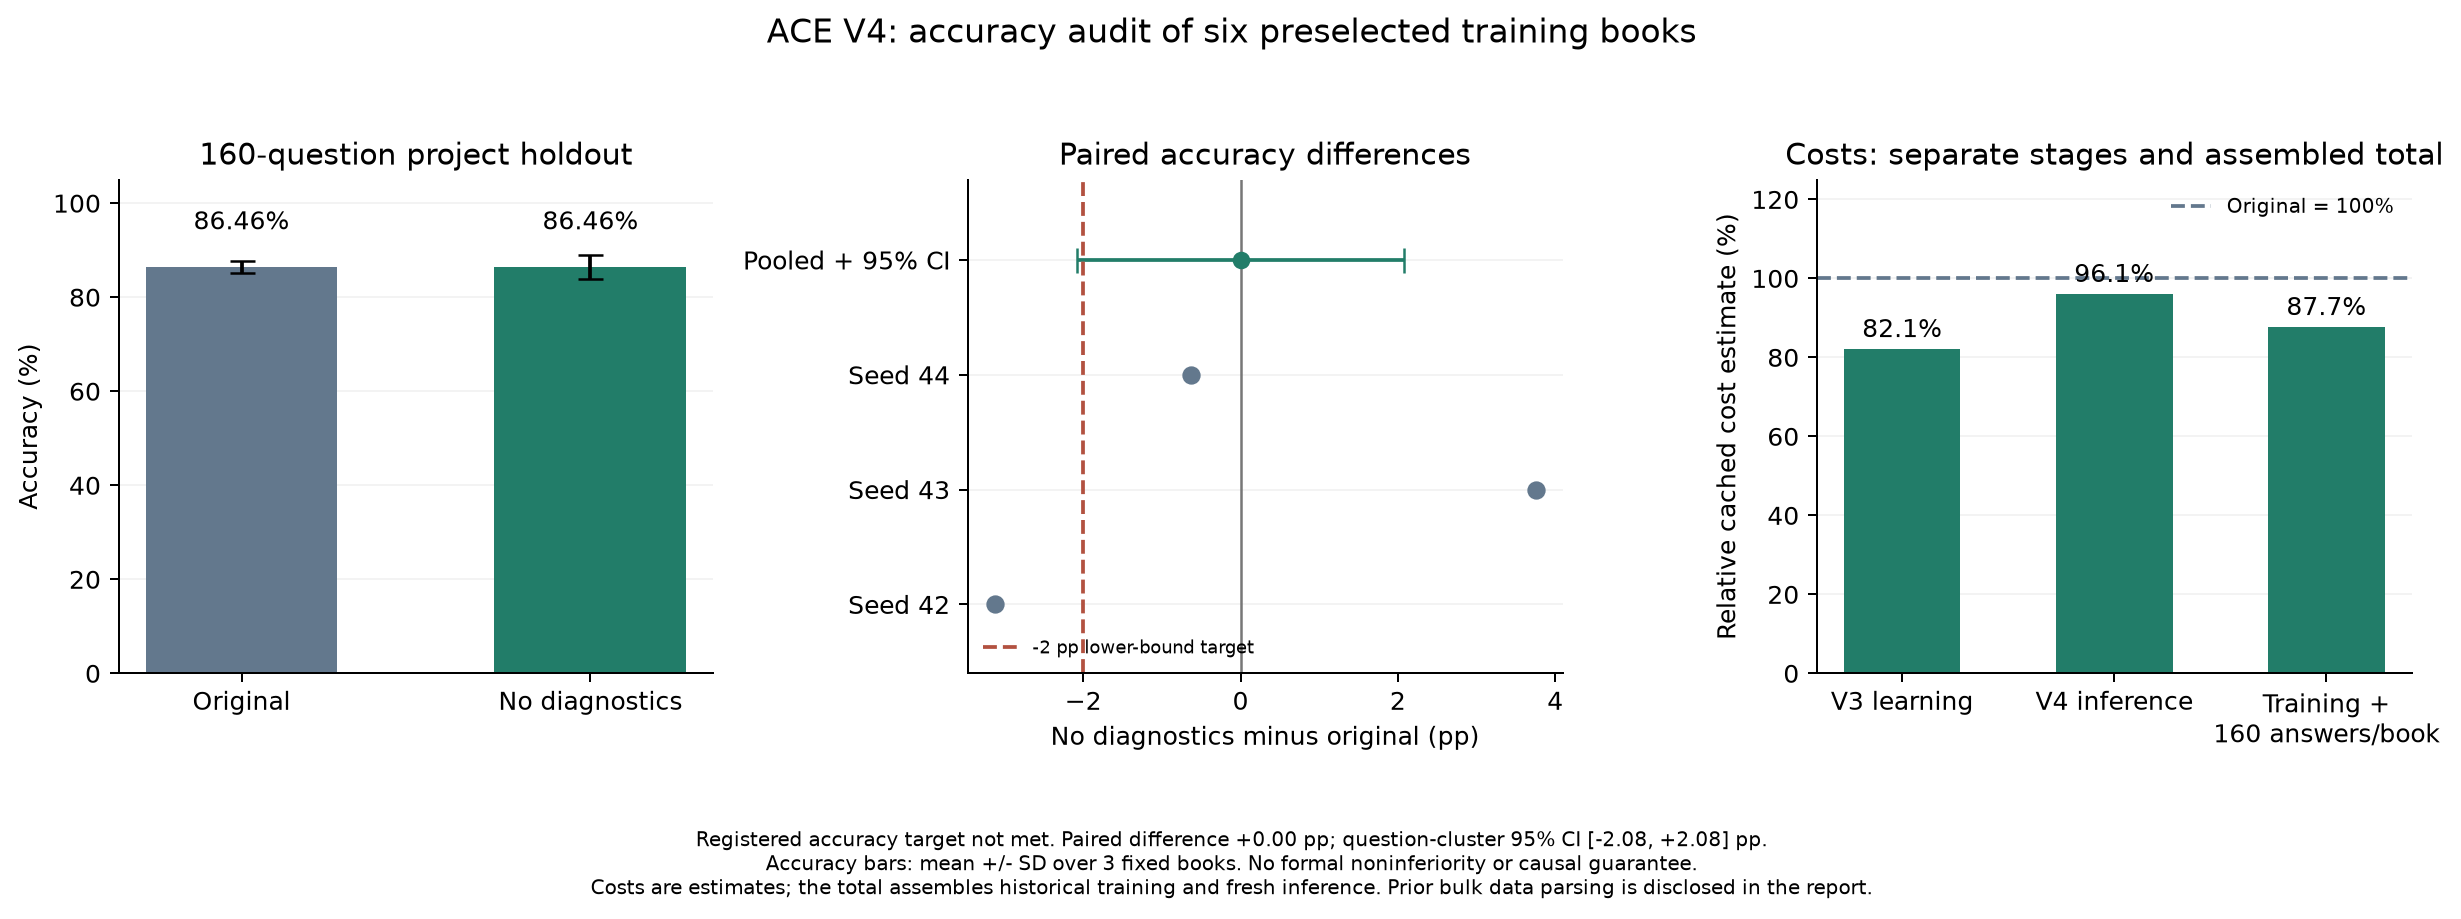
\includegraphics[width=\linewidth]{figures/v4_results.png}
\caption{Fixed-book accuracy, paired differences and relative estimated costs. The pooled interval clusters by question; per-seed bars are descriptive. The dashed $-2\pp$ reference is the predefined interval criterion.}
\end{figure}
The mean difference is $0.00\pp$, with a question-clustered 95\% interval of $[-2.0833,+2.0833]\pp$. The lower-bound criterion fails without rounding or changing the threshold. Cache-aware inference accounting decreases by 3.92\%. All truncated responses remain in the denominator.

Of 480 paired answers, 16 change from original-correct to diagnostic-free-wrong and 16 in the reverse direction. Thus, the equal mean does not imply identical behavior. The evidence shows no net observed accuracy change, but lacks the precision required by the predefined criterion. It neither proves degradation nor proves accuracy preservation. No threshold adjustment, additional rule tuning or selective retesting follows the result.

\clearpage
\section{Auxiliary Experiments and Debug Diary}
\subsection{Additional efficiency proposals}
\begin{table}[h!]
\centering\smalltable
\begin{tabularx}{\linewidth}{P{34mm}Y P{42mm}}
\toprule
Proposal & Key result & Interpretation \\
\midrule
Selective / retrieval & Test A: 79.67\% / 81.33\%; combined: 82.33\% & Below ACE (84.00\%) \\
Brief output (V2) & Accuracy: $-1.00\pp$; cache-aware cost: $-42.12\%$ & Accuracy inconclusive \\
Routing (V3) & Dev accuracy: $+3.33\pp$; cost: $-5.63\%$ & 15\% cost gate failed \\
\bottomrule
\end{tabularx}
\caption{Auxiliary results, compared with the original condition in each study.}
\end{table}
On test B, original and brief-output accuracies are 80.67\% and 79.67\%, respectively; the difference is $-1.00\pp$ (95\% CI $[-4.33,+2.00]\pp$). Five format fallbacks recover no correct answers.

The brief-output policy keeps the full playbook, adds a soft 60-word reasoning instruction, and makes at most one original-prompt fallback when the answer is nonnumeric or nonfinite. It retains the 4,096-token hard cap. Screening on 20 questions and confirmation on 40 precede the disjoint second 100-question official test. The V3 router uses pre-generation question features and defaults to original output. It is selected on 40 development questions using grouped four-fold cross-validation. Its best 5.63\% cost saving falls short of the 15\% gate, so routing is not evaluated on the 160-question holdout. Development gains are not independent test evidence. Neither study establishes an accuracy-preserving improvement.

\subsection{Operational and evaluation issues}
\begin{table}[h!]
\centering\smalltable
\begin{tabularx}{\linewidth}{P{29mm}Y Y}
\toprule
Issue & Action & Qualification \\
\midrule
Truncation & Retain nonempty output & Fixed denominator \\
API failures & Bounded recovery & Unknown billing retained \\
Units / labels & Preserve original scoring & No post-hoc correction \\
Cache effects & Report both cost metrics & Estimates, not bills \\
Validation loading & Disclose parsing deviation & Audit model prompts \\
\bottomrule
\end{tabularx}
\caption{Debugging actions and remaining limits.}
\end{table}
The initial transport rejected nonempty truncated responses; it was corrected to retain the text and finish reason, matching upstream behavior without increasing the output cap. Completed outputs survive API failures. Explicit HTTP 503 errors receive bounded recovery; HTTP 402, credential or budget problems stop execution. Twelve historical unknown-billing requests remain reserved, and provider interruption does not explain every local failure.

Case inspection covered percentage/decimal units and simple/compound interest; released labels and scoring were not changed. Cache-aware and standardized costs are both reported because fewer tokens need not imply lower cached cost. Public usage, audits and phase summaries are retained; raw response archives are excluded.

The complete project accounting estimate is CNY 39.8473, including retained historical failure reserves. V4 itself completes 960 requests without a network failure and retains 14 nonempty truncated outputs. This documents the observed run, not guaranteed service reliability.

\clearpage
\section{Limitations, Reproducibility Package, and Conclusions}
\label{sec:limits}
\textbf{Scope and generalization.} Findings concern one Formula subset, one hosted-model alias and three training orders. The experiment does not test all ACE applications, new model families or arbitrary future retraining. Temperature zero and order seeds do not make hosted inference deterministic. The current alias does not pin immutable model weights.

\textbf{Data boundary.} V3's frozen loader decoded the full validation JSONL before selecting the original 30 validation examples. This deviates from a strict ``never loaded'' claim. Audited training/validation prompts contain only the original 60/30 examples; the 160 questions did not guide routing selection. V4 selects line IDs before JSON parsing, constructs model inputs without target fields, and audits all 960 prompts against the specified template, book and question. Selected raw records still contain labels when decoded before masking. Therefore, this is a validation-derived project holdout with a disclosed parsing deviation, not a pristine new official test or a process that never decoded labels.

\textbf{Statistical and causal scope.} The main intervals capture question sampling conditional on fixed books. Three live pairs do not isolate every effect of server randomness, caching and condition order. The failed V4 interval criterion is reported unchanged. Multiple auxiliary analyses and the evolving report focus limit broad confirmatory claims.

\begin{table}[h!]
\centering\smalltable
\begin{tabularx}{\linewidth}{P{39mm}Y P{38mm}}
\toprule
Location & Contents & Use \\
\midrule
\art{report/} & LaTeX, figures, references, PDF & Compile the report \\
Configs / contracts & Frozen parameters and hashes & Inspect the protocol \\
\art{repro/artifacts/} & Predictions, usage, books, analyses & Recompute V2/V3/V4 \\
\art{README.md}, commits & Setup, commands, attribution & Install and run \\
Private archives & Original raw responses & Local-only replay \\
\bottomrule
\end{tabularx}
\caption{Package contents and verification routes.}
\end{table}
Public V2/V3/V4 recomputation requires neither API keys nor private logs. Full trajectory replay depends on excluded local archives; new hosted execution incurs API costs. Build and run commands are provided in the root README. Zoom presentation preparation remains outside this delivery.

\textbf{Conclusions.} RQ1 is supported as a behavioral reproduction: ACE improves over the empty-playbook Generator by $14.67\pp$ on the first test cohort. For RQ2, the isolated diagnostic removal preserves all replayed learning states and produces lower aggregate learning calls, cost estimates and median workflow time in fresh runs. RQ3 remains unresolved at the predefined precision: equal holdout accuracy is compatible with meaningful differences, and the interval criterion fails. Future users should distinguish learning from measurement overhead, preserve test boundaries, and evaluate cache-aware cost together with quality. The present evidence supports a measured engineering optimization with explicit uncertainty, rather than a lossless-learning guarantee.

\vspace{-2mm}
{\small\setlength{\bibsep}{2pt}\bibliographystyle{plainnat}\bibliography{references}}
\end{document}
